\documentclass[xcolor={table}]{beamer}
\usepackage{fleqn}
\usepackage{graphicx}
\usepackage{coordsys} %for \numbline commander

%Setup appearance:
\usetheme{Darmstadt}
\usefonttheme[onlylarge]{structurebold}
\setbeamerfont*{frametitle}{size=\normalsize,series=\bfseries}
\setbeamertemplate{navigation symbols}{}
\setbeamertemplate{bibliography item}{[\theenumiv]}

% Standard packages
\usepackage[english]{babel}
\usepackage[latin1]{inputenc}
\usepackage{times}
\usepackage[T1]{fontenc}
\usepackage{multirow}
\usepackage{subfigure}
\usepackage{pbox}
\usepackage{arydshln}
\usepackage{pifont}
\usepackage{cancel}
\usepackage{rotating} % for sideways headings

% Source Code packages
\usepackage{algorithm2e}
\usepackage{algorithmic}

\DeclareSymbolFont{extraup}{U}{zavm}{m}{n}
\DeclareMathSymbol{\varclub}{\mathalpha}{extraup}{84}
\DeclareMathSymbol{\varspade}{\mathalpha}{extraup}{85}
\DeclareMathSymbol{\varheart}{\mathalpha}{extraup}{86}
\DeclareMathSymbol{\vardiamond}{\mathalpha}{extraup}{87}

%%% This section command that adds a big page with section dividers
\usepackage{xifthen}% provides \isempty test
\newcommand{\SectionSlide}[2][]{
	\ifthenelse{\isempty{#1}}
		{\section{#2}\begin{frame} \begin{center}\begin{huge}#2\end{huge}\end{center}\end{frame}}
		{\section[#1]{#2}\begin{frame} \begin{center}\begin{huge}#2\end{huge}\end{center}\end{frame}}
}
%Extends the section slide to to include a shortened section title for the navigation bar as a second parameter
\newcommand{\SectionSlideShortHeader}[3][]{
	\ifthenelse{\isempty{#1}}
		{\section[#3]{#2}\begin{frame} \begin{center}\begin{huge}#2\end{huge}\end{center}\end{frame}}
		{\section[#1]{#2}\begin{frame} \begin{center}\begin{huge}#3\end{huge}\end{center}\end{frame}}
}

\newcommand{\refer}[1]{\footnote{#1}}
\newcommand{\GW}{\text{\textit{Guess-Who~}}}
\newcommand{\keyword}[1]{\alert{\textbf{#1}}\index{#1}}
\newcommand{\firstkeyword}[1]{\textbf{#1}\index{#1}}
\newcommand{\indexkeyword}[1]{\alert{\textbf{#1}\index{#1}}}
\newcommand{\featN}[1]{\textsc{#1}}
\newcommand{\featL}[1]{\textit{'#1'}}
 \newcommand{\ourRef}[1]{\ref{#1} $^{\text{\tiny[\pageref{#1}]}}$}
 \newcommand{\ourEqRef}[1]{\eqref{#1}$^{\text{\tiny[\pageref{#1}]}}$}
  
\DeclareMathOperator*{\argmax}{argmax}
\DeclareMathOperator*{\argmin}{argmin}



\title{Probability-based Learning\\Sections $6.1, 6.2, 6.3$}
	\author{John D. Kelleher and Brian Mac Namee and Aoife D'Arcy}
	\institute{}
	\date{}

	
\begin{document}
\begin{frame}
	\titlepage
\end{frame}
\begin{frame}
	 \tableofcontents
\end{frame}
\SectionSlide{Big Idea}

 \begin{frame} [plain]
\begin{figure}
\centering
\subfigure[]{\label{fig:3cardTrickFan}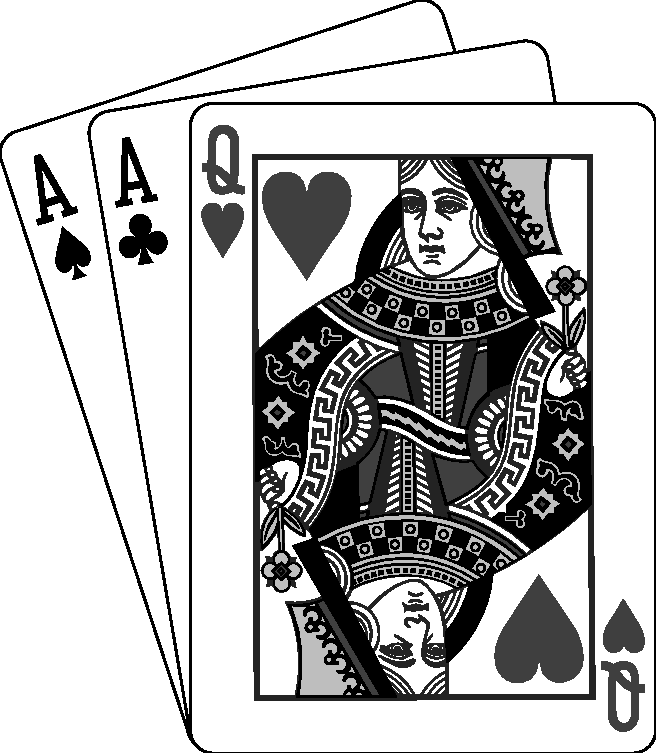
\includegraphics[width=0.29\textwidth]{./images/cardfan2BW.pdf}} \\
\subfigure[]{\label{fig:3cardTrickCards1}
\includegraphics[width=0.2\textwidth]{./images/Blue_Back_BW_3.pdf}

\includegraphics[width=0.2\textwidth]{./images/Blue_Back_BW_3.pdf}

\includegraphics[width=0.2\textwidth]{./images/Blue_Back_BW_3.pdf}}
\caption{A game of \textit{find the lady}}
\label{fig:3cardTrick1}
\end{figure}
\end{frame} 

 \begin{frame} [plain]
\begin{figure}
\centering
\subfigure[]{\label{fig:3cardTrickCards1}
\includegraphics[width=0.2\textwidth]{./images/Blue_Back_BW_3.pdf}

\includegraphics[width=0.2\textwidth]{./images/Blue_Back_BW_3.pdf}

\includegraphics[width=0.2\textwidth]{./images/Blue_Back_BW_3.pdf}} \\
\subfigure[]{\label{fig:3cardTrickBars1}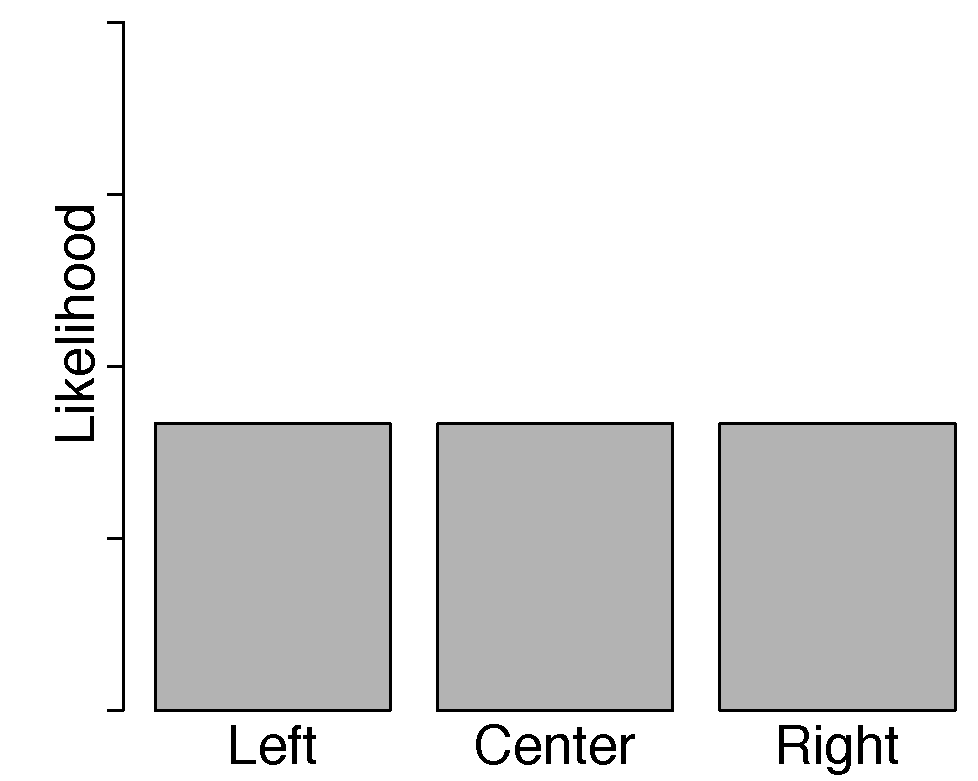
\includegraphics[width=0.34\textwidth]{./images/findTheLadyBarPlot1.pdf}}
\caption{A game of \textit{find the lady}: (a) the cards dealt face down on a table; and (b) the initial likelihoods of the queen ending up in each position.}
\label{fig:3cardTrick2}
\end{figure}
\end{frame} 

 \begin{frame} [plain]
\begin{figure}
\centering
\subfigure[]{\label{fig:3cardTrickCards1}
\includegraphics[width=0.2\textwidth]{./images/Blue_Back_BW_3.pdf}

\includegraphics[width=0.2\textwidth]{./images/Blue_Back_BW_3.pdf}

\includegraphics[width=0.2\textwidth]{./images/Blue_Back_BW_3.pdf}} \\
\subfigure[]{\label{fig:3cardTrickBars1}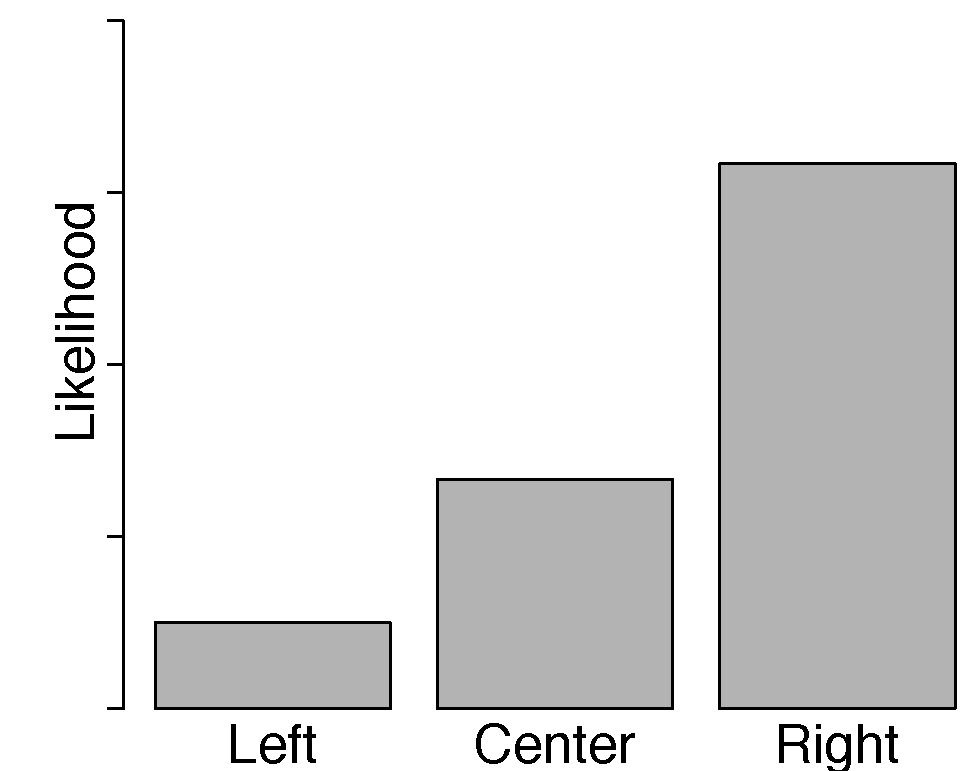
\includegraphics[width=0.34\textwidth]{./images/findTheLadyBarPlot2.pdf}}
\caption{A game of \textit{find the lady}: (a) the cards dealt face down on a table; and (b) a revised set of likelihoods for the position of the queen based on evidence collected.}
\label{fig:3cardTrick3}
\end{figure}
\end{frame} 

 \begin{frame} [plain]
\begin{figure}
\centering
\subfigure[]{\label{fig:3cardTrickCards1}
\includegraphics[width=0.2\textwidth]{./images/Blue_Back_BW_3.pdf}

\includegraphics[width=0.2\textwidth]{./images/Blue_Back_BW_3.pdf}
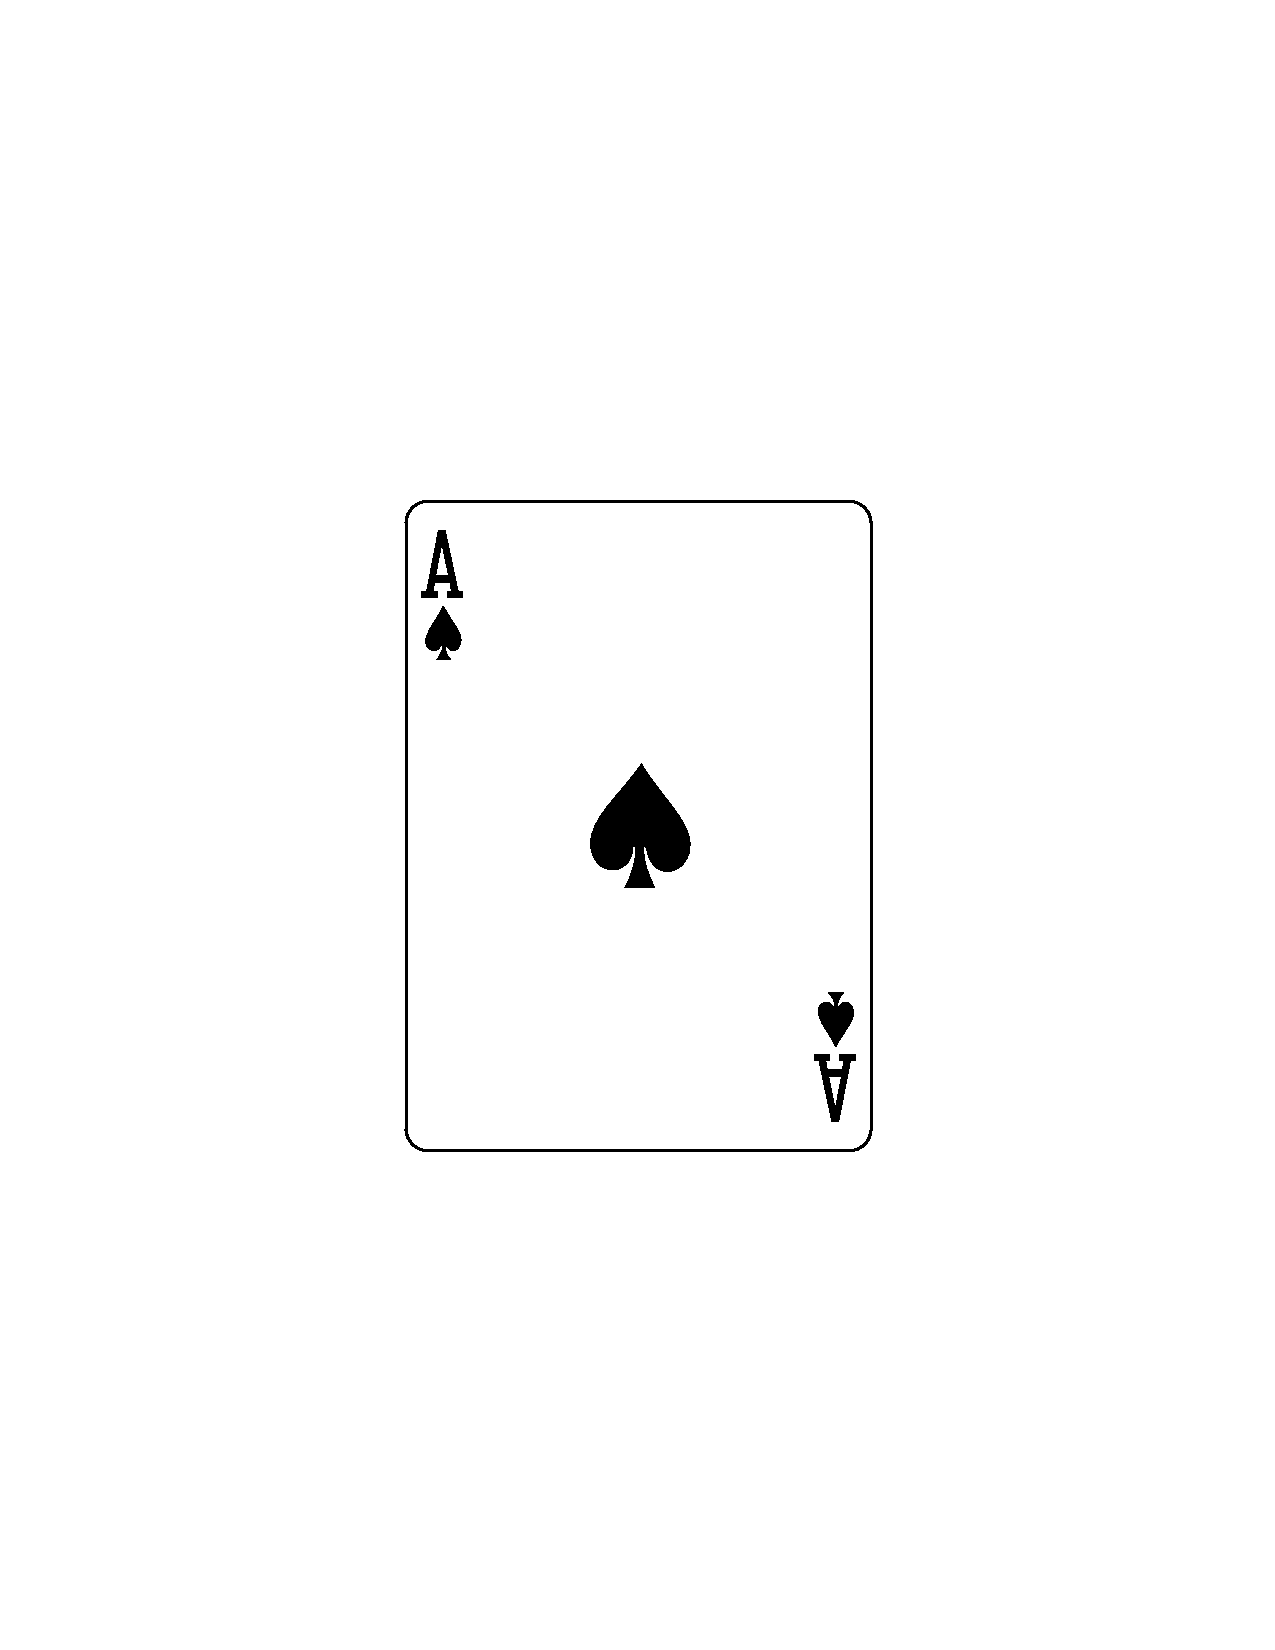
\includegraphics[width=0.2\textwidth]{./images/AS.pdf}} \\
\subfigure[]{\label{fig:3cardTrickBars1}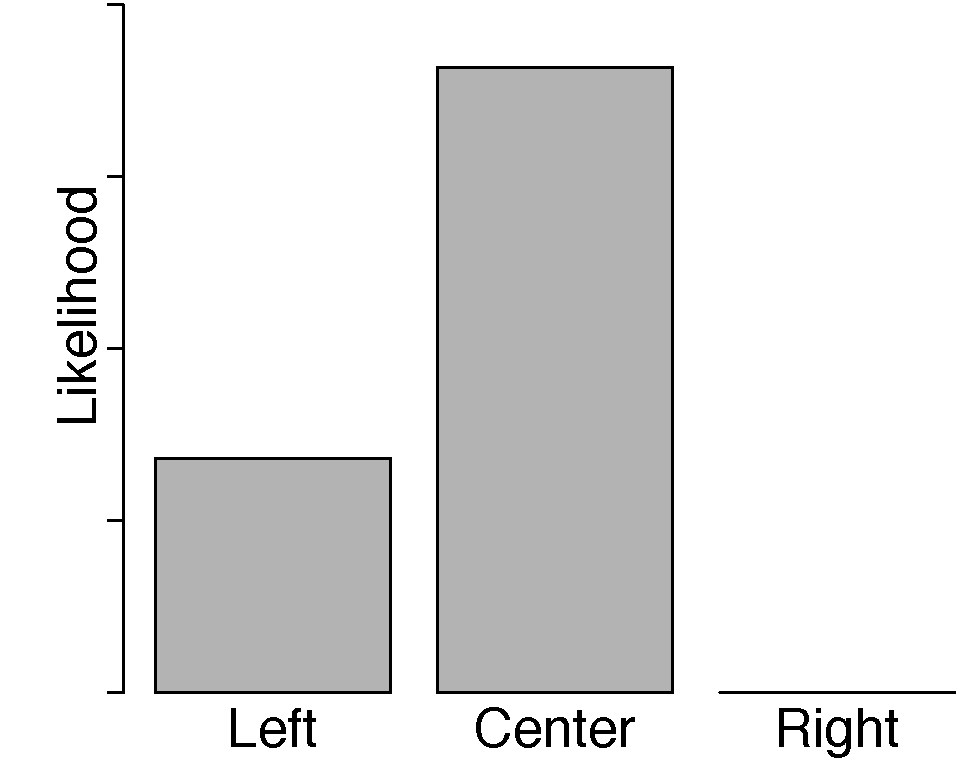
\includegraphics[width=0.34\textwidth]{./images/findTheLadyBarPlot3.pdf}}
\caption{A game of \textit{find the lady}: (a) The set of cards after the wind blows over the one on the right; (b) the revised likelihoods for the position of the queen based on this new evidence.}
\label{fig:3cardTrick4}
\end{figure}
\end{frame} 

 \begin{frame} [plain]
\begin{figure}
\centering
\label{fig:3cardTrickCards4}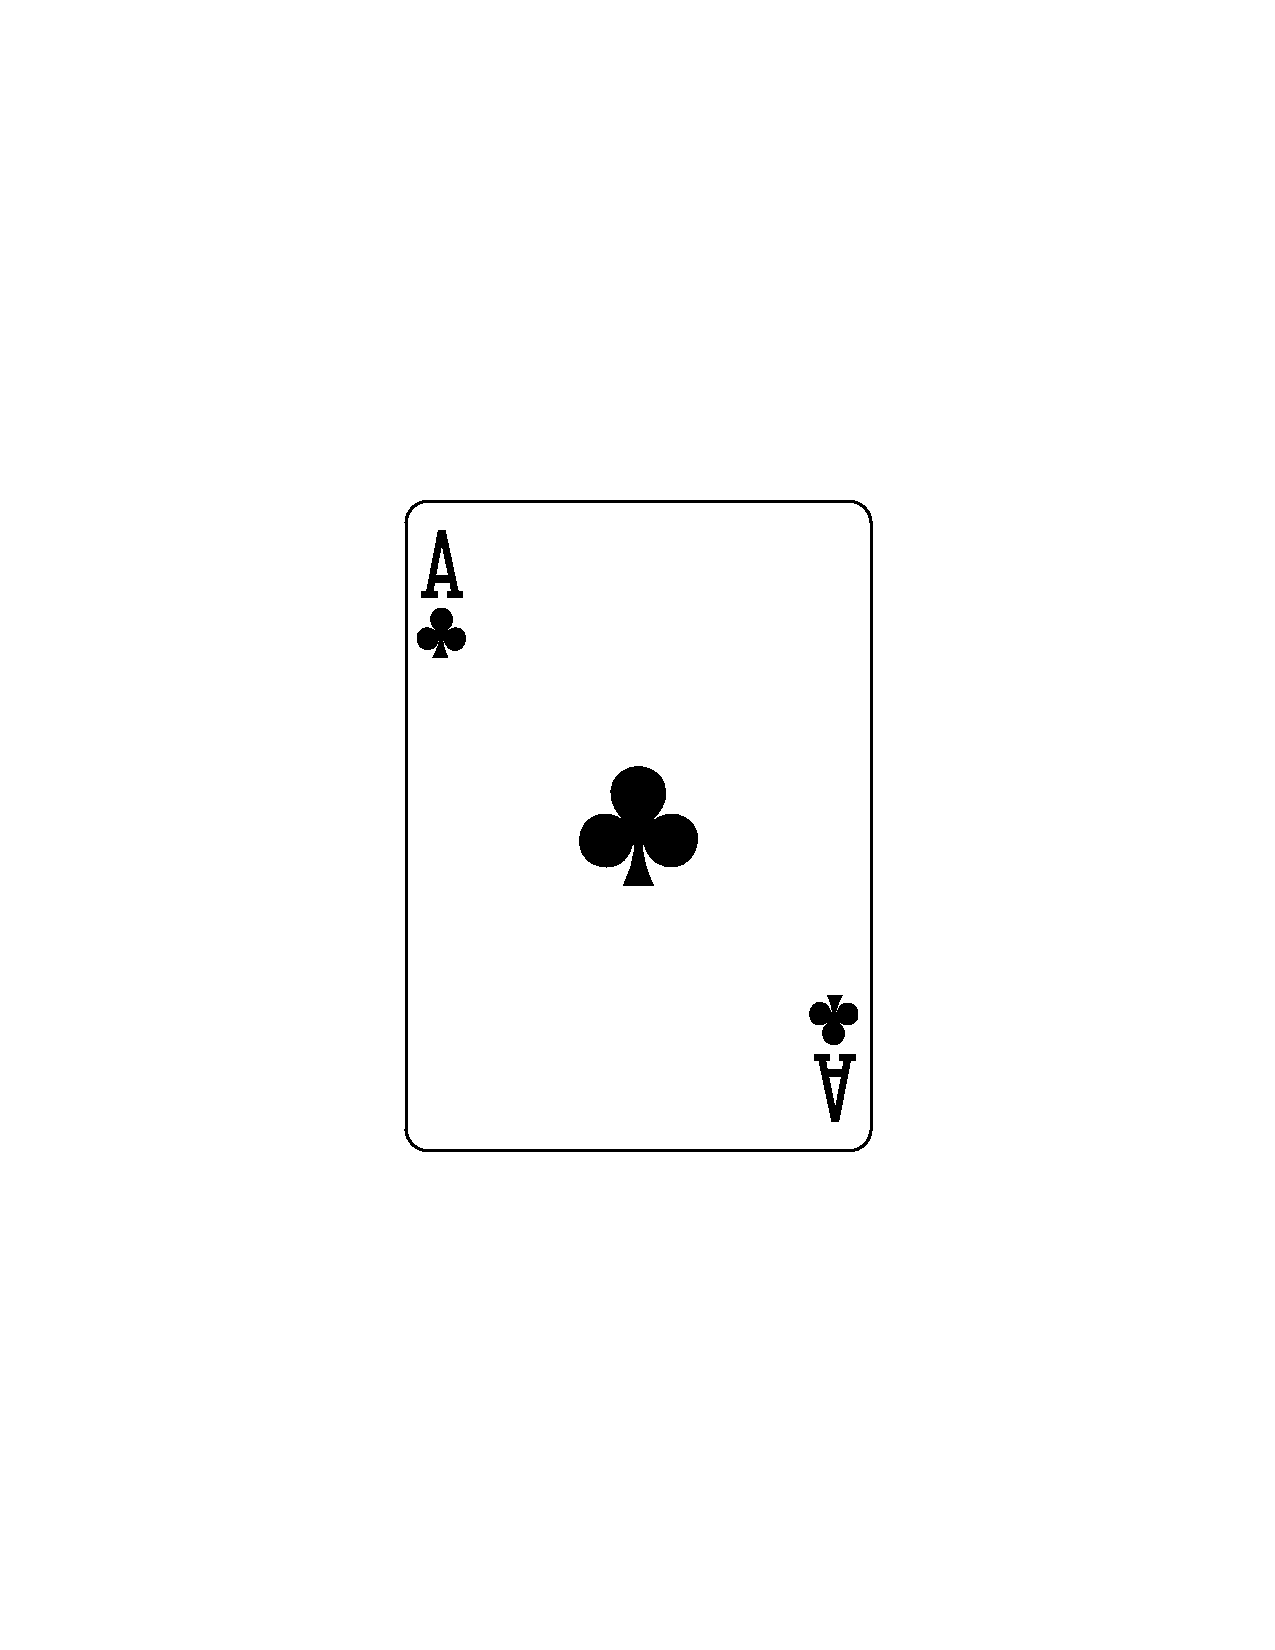
\includegraphics[width=0.2\textwidth]{./images/AC.pdf}
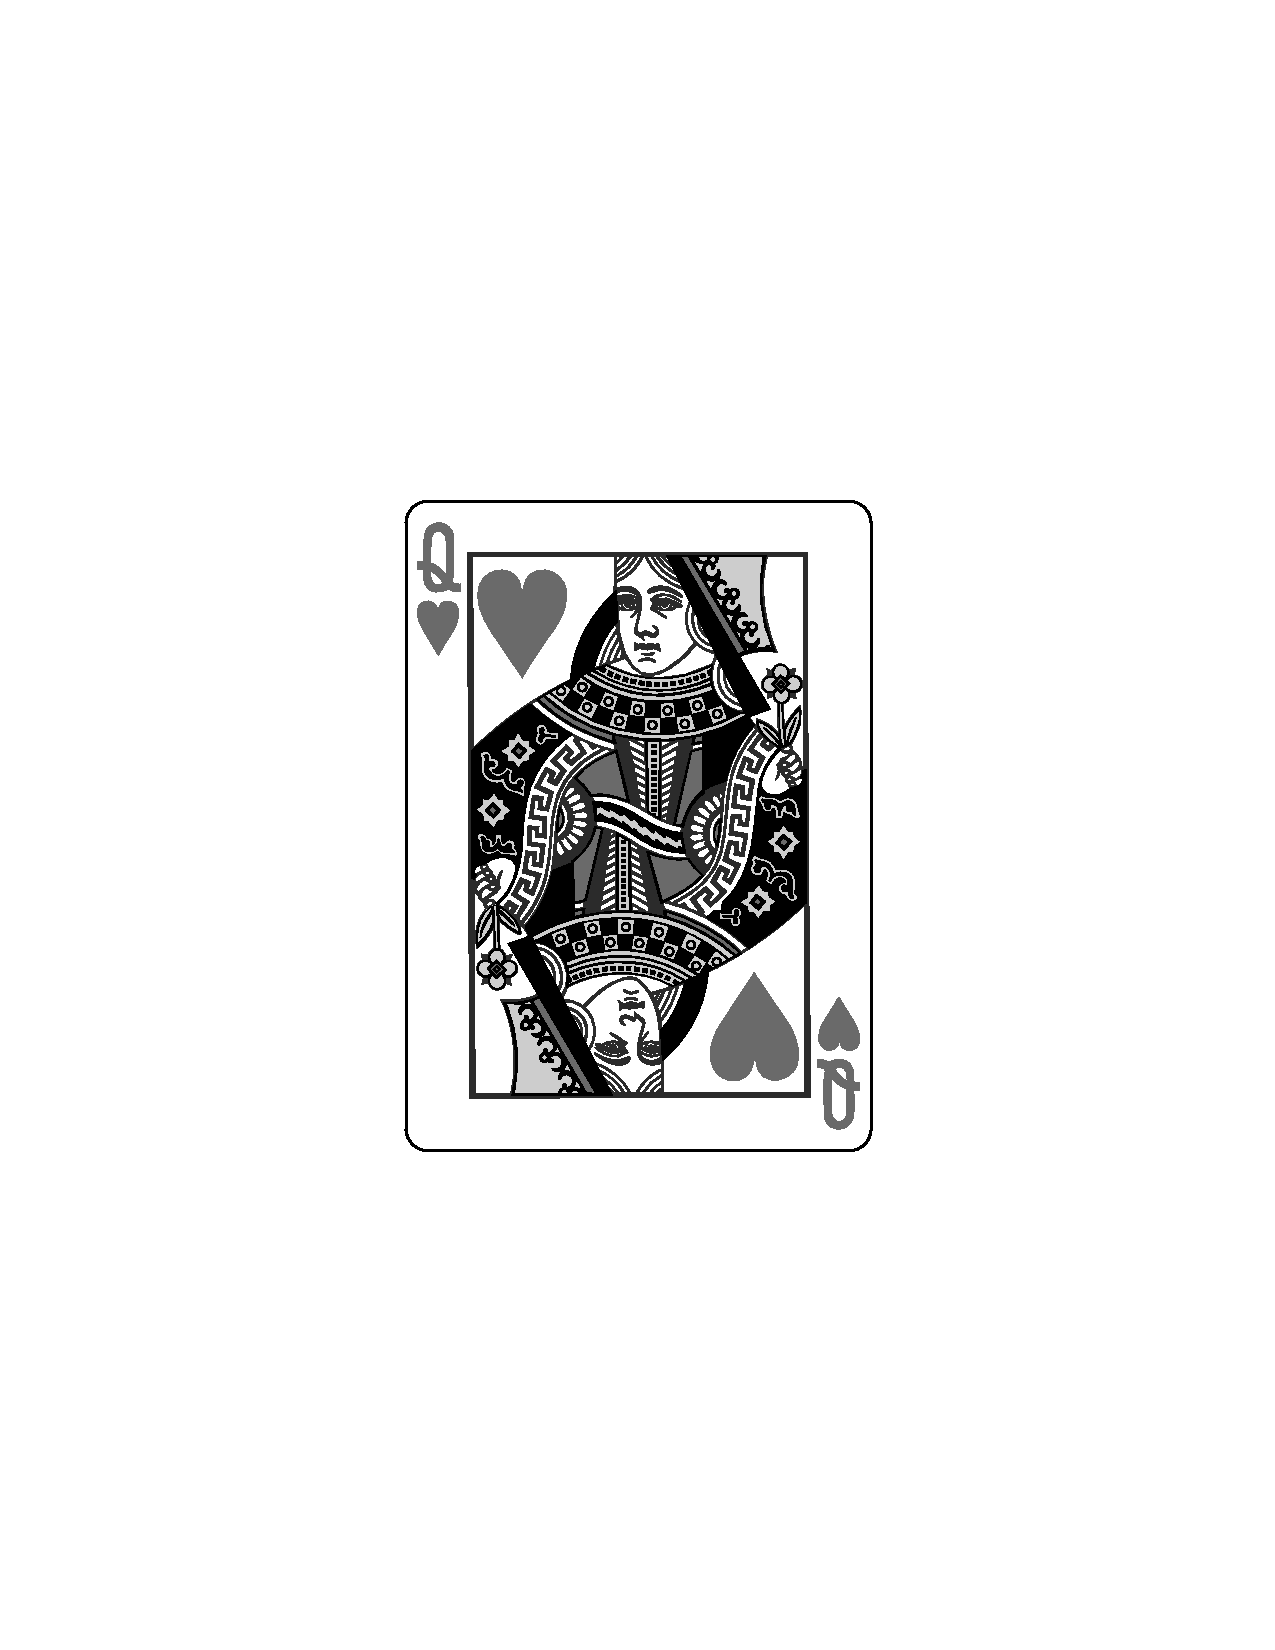
\includegraphics[width=0.2\textwidth]{./images/QH_BW.pdf}
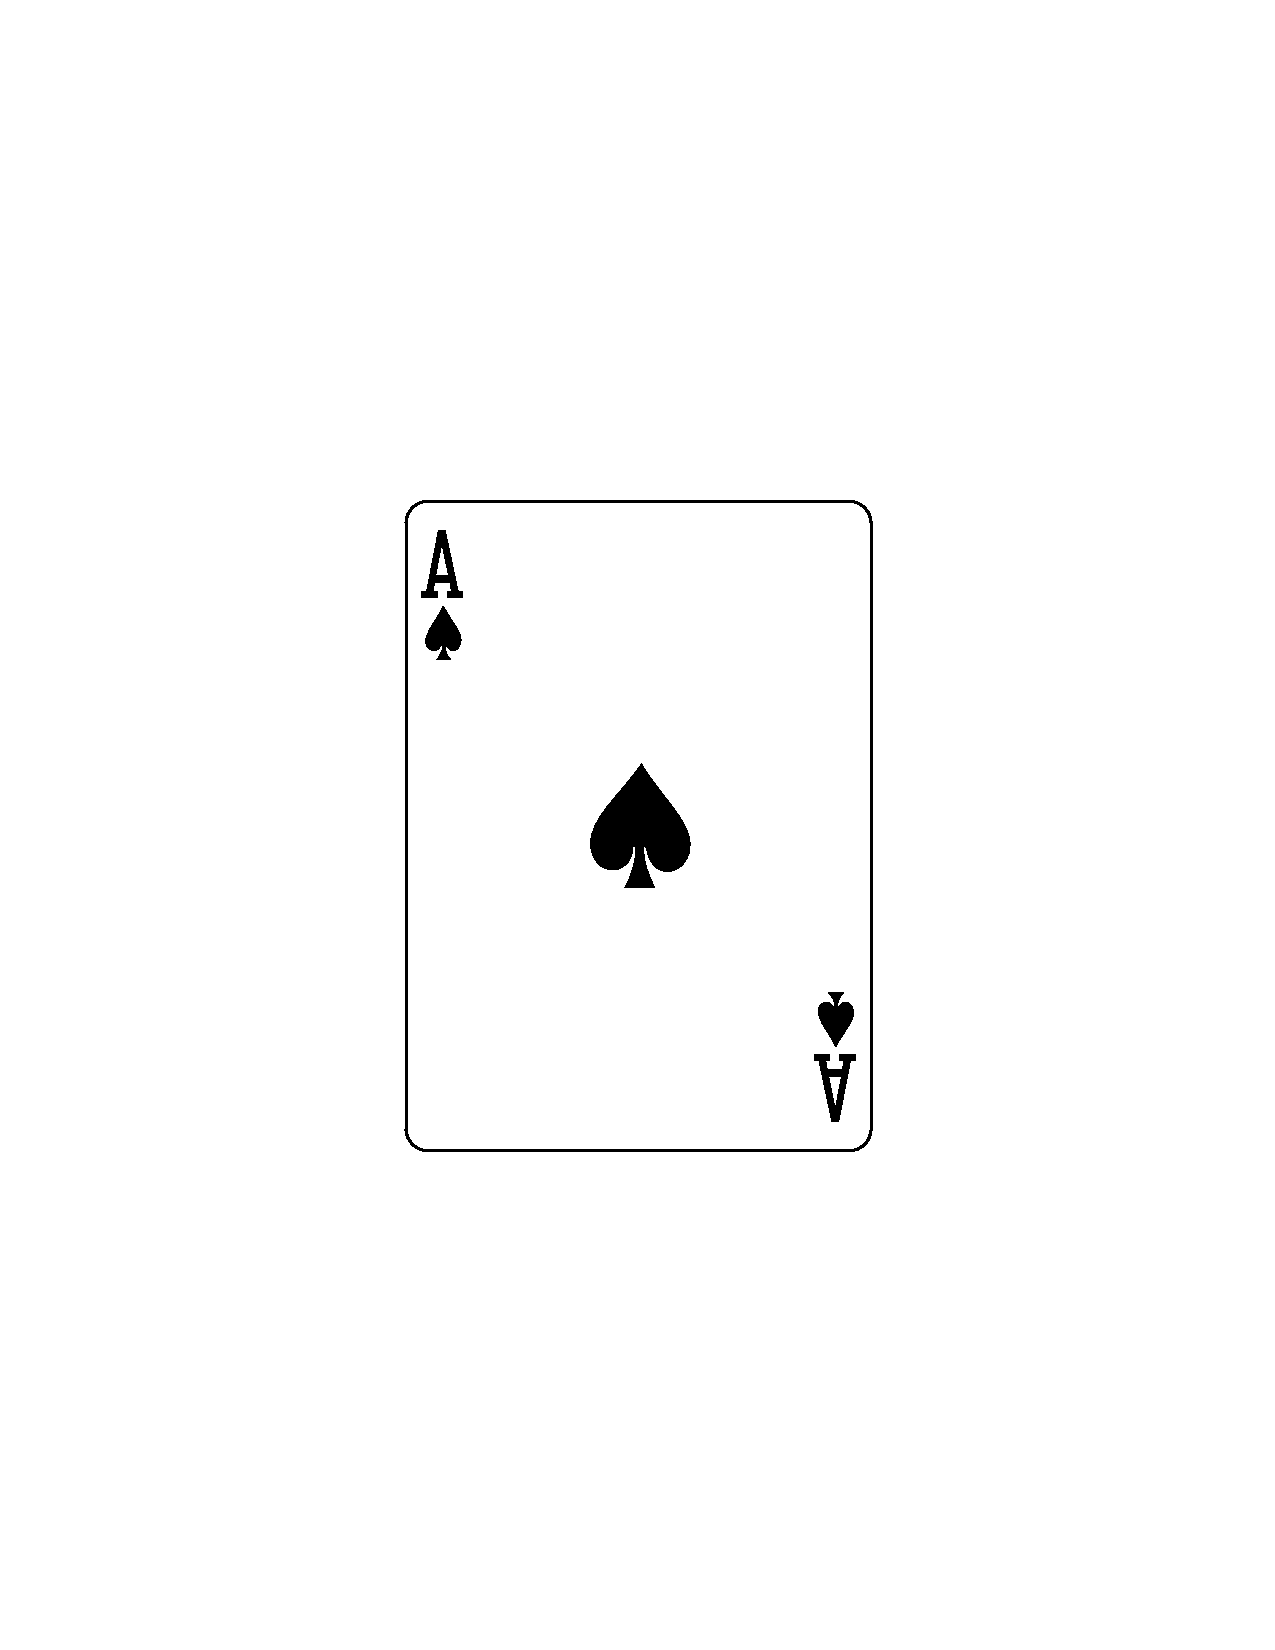
\includegraphics[width=0.2\textwidth]{./images/AS.pdf}
\caption{A game of \textit{find the lady}: The final positions of the cards in the game.}
\label{fig:3cardTrick5}
\end{figure}
\end{frame} 

\begin{frame}
	\begin{alertblock}{Big Idea}
		\begin{itemize}
			\item We can use estimates of likelihoods to determine the most likely prediction that should be made.
			\item More importantly, we revise these predictions based on data we collect and whenever extra evidence becomes available.
		\end{itemize}
	\end{alertblock}
\end{frame}

\SectionSlide{Fundamentals}

 \begin{frame} 
\begin{table}[!tb]
\caption{A simple dataset for \featN{Meningitis} diagnosis with descriptive features that describe the presence or absence of three common symptoms of the disease: \featN{Headache}, \featN{Fever}, and \featN{Vomiting}.}
\label{table:probExample1}
\centering
\begin{footnotesize}
\begin{tabular}{ccccc}
\hline
\featN{ID} & \featN{Headache} & \featN{Fever} & \featN{Vomiting} & \featN{Meningitis}\\
\hline
1 & true & true & false & false\\
2 & false & true & false & false\\
3 & true & false & true & false\\
4 & true & false & true & false\\
5 & false & true & false & true\\
6 & true & false & true & false\\
7 & true & false & true & false\\
8 & true & false & true & true\\
9 & false & true & false & false\\
10 & true & false & true & true\\
\hline
\end{tabular}
\end{footnotesize}
\end{table}
\end{frame} 


\begin{frame} 
\begin{itemize}
\item A \keyword{probability function}, $P()$, returns the probability of a feature taking a specific value.
\item A \keyword{joint probability} refers to the probability of an assignment of specific values to multiple different features.
\item A \keyword{conditional probability}  refers to the probability of one feature taking a specific value given that we already know the value of a different feature
\item A \keyword{probability distribution} is a data structure that describes the probability of each possible value a feature can take. The sum of a probability distribution must equal $1.0$.
\end{itemize}
\end{frame} 

\begin{frame} 
\begin{itemize}
\item A \keyword{joint probability distribution} is a probability distribution over more than one feature assignment and is written as a multi-dimensional matrix in which each cell lists the probability of a particular combination of feature values being assigned. 
\item The sum of all the cells in a joint probability distribution must be $1.0$. 
\end{itemize}
\end{frame} 

 \begin{frame} 
\begin{equation*}
\mathbf{P}(H,F,V,M) = \left[ \begin{array}{ll} 
P(h, f, v, m),& P(\lnot h, f, v, m)\\
P(h, f, v, \lnot m),& P(\lnot h, f, v, \lnot m)\\
P(h, f, \lnot v, m),& P(\lnot h, f, \lnot v, m)\\
P(h, f, \lnot v, \lnot m),& P(\lnot h, f, \lnot v, \lnot m)\\
P(h, \lnot f, v, m),& P(\lnot h, \lnot f, v, m)\\
P(h, \lnot f, v, \lnot m),& P(\lnot h, \lnot f, v, \lnot m)\\
P(h, \lnot f, \lnot v, m),& P(\lnot h, \lnot f, \lnot v, m) \\
P(h, \lnot f, \lnot v, \lnot m),& P(\lnot h, \lnot f, \lnot v, \lnot m) \\ \end{array} \right]
\label{eq:jointprobABC}
\end{equation*}
\end{frame} 

\begin{frame} 
\begin{itemize}
\item Given a joint probability distribution, we can compute the probability of any event in the domain that it covers by summing over the cells in the distribution where that event is true. 
\item Calculating probabilities in this way is known as \keyword{summing out}. 
\end{itemize}
\end{frame} 

\subsection{Bayes' Theorem}

 \begin{frame} 
\begin{alertblock}{Bayes' Theorem}
\begin{equation*}
P(X|Y)=\frac{P(Y|X)P(X)}{P(Y)}
\end{equation*}
\end{alertblock}
\end{frame} 


\begin{frame}
	\begin{example}
	After a yearly checkup, a doctor informs their patient that he has both bad news and good news. The bad news is that the patient has tested positive for a serious disease and that the test that the doctor has used is $99\%$ accurate (i.e., the probability of testing positive when a patient has the disease is 0.99, as is the probability of testing negative when a patient does not have the disease). The good news, however, is that the disease is extremely rare, striking only 1 in 10,000 people. 
	\end{example}
	\begin{itemize}
		\item  What is the actual probability that the patient has the disease? 
		\item Why is the rarity of the disease good news given that the patient has tested positive for it?
	\end{itemize}
\end{frame}

 \begin{frame}
 \begin{equation*}
P(d|t)=\frac{P(t|d)P(d)}{\alert{P(t)}}
\end{equation*}
\begin{eqnarray*}
P(t) & = & P(t|d)P(d)+P(t|\lnot d)P(\lnot d) \\
& = & (0.99 \times 0.0001)+(0.01 \times 0.9999) = 0.0101
\end{eqnarray*}
\begin{eqnarray*}
P(d|t)& = &\displaystyle\frac{0.99 \times 0.0001}{0.0101} \\
& = & 0.0098
\end{eqnarray*}
\end{frame} 

 \begin{frame} 
 Deriving Bayes theorem
\begin{equation*}
P(Y|X)P(X)=P(X|Y)P(Y)
\end{equation*}
\begin{equation*}
\frac{P(X|Y)P(Y)}{P(Y)}~=~\frac{P(Y|X)P(X)}{P(Y)}
\end{equation*}
\begin{alignat*}{4}
& \frac{P(X|Y)\cancel{P(Y)}}{\cancel{P(Y)}}&~=~&\frac{P(Y|X)P(X)}{P(Y)}\\
\Rightarrow & P(X|Y)&~=~&\frac{P(Y|X)P(X)}{P(Y)}
\end{alignat*}
\end{frame} 






 \begin{frame}
 \begin{itemize}
 	\item The divisor is the prior probability of the evidence
	\item This division functions as a normalization constant.
\end{itemize} 
\begin{eqnarray*}
0 \leq P(X|Y) &\leq & 1\\
\sum_{i} P(X_i|Y) & =  & 1.0
\end{eqnarray*}
\end{frame}




\begin{frame}
\begin{itemize}
	\item We can calculate this divisor directly from the dataset.
\end{itemize} 
\begin{equation*}
P(Y)=\frac{|\{ \text{rows where Y is the case} \}|}{|\{ \text{rows in the dataset} \}|}
\label{eq:denomFromData}
\end{equation*}
\begin{itemize}
	\item Or, we can use the \keyword{Theorem of Total Probability} to calculate this divisor.
\end{itemize} 
\begin{equation}
P(Y)=\sum_i P(Y|X_i)P(X_i)
\label{eq:totProb2}
\end{equation}
\end{frame} 

\subsection{Bayesian Prediction}

\begin{frame}
	\begin{alertblock}{Generalized Bayes' Theorem}
\begin{equation*}
P(t=l|\mathbf{q}[1],\dots,\mathbf{q}[m])=\frac{P(\mathbf{q}[1],\dots,\mathbf{q}[m]| t=l)P(t=l)}{P(\mathbf{q}[1],\dots,\mathbf{q}[m])}
\end{equation*}
\end{alertblock}
\end{frame}

\begin{frame}
	\begin{block}{Chain Rule}
\begin{equation*}
\begin{alignedat}{2}
P(\mathbf{q}[1],& \dots, \mathbf{q}[m])= \\
&P(\mathbf{q}[1]) \times P(\mathbf{q}[2] | \mathbf{q}[1]) \times\\
& \dots \times P(\mathbf{q}[m] |\mathbf{q}[m-1], \dots, \mathbf{q}[2],\mathbf{q}[1])
\end{alignedat}
\end{equation*}
	\end{block}
	\begin{itemize}
	\item To apply the chain rule to a conditional probability we just add the conditioning term to each term in the expression: 
	\end{itemize}
\begin{equation*}
\begin{alignedat}{2}
P(\mathbf{q}[1],&\dots,\mathbf{q}[m] |\alert{t=l})= \\
&P(\mathbf{q}[1]|\alert{t=l}) \times P(\mathbf{q}[2] | \mathbf{q}[1], \alert{t=l}) \times \dots\\
& \dots\times P(\mathbf{q}[m] |\mathbf{q}[m-1], \dots, \mathbf{q}[3], \mathbf{q}[2],\mathbf{q}[1], \alert{t=l})
\end{alignedat}
\end{equation*}
\end{frame}


 \begin{frame} 
\begin{table}[!tb]
\centering
\begin{footnotesize}
\begin{tabular}{ccccc}
\hline
\featN{ID} & \featN{Headache} & \featN{Fever} & \featN{Vomiting} & \featN{Meningitis}\\
\hline
1 & true & true & false & false\\
2 & false & true & false & false\\
3 & true & false & true & false\\
4 & true & false & true & false\\
5 & false & true & false & true\\
6 & true & false & true & false\\
7 & true & false & true & false\\
8 & true & false & true & true\\
9 & false & true & false & false\\
10 & true & false & true & true\\
\hline
\end{tabular}
\end{footnotesize}
\end{table}
 \begin{table}
\centering
\begin{footnotesize}
\begin{tabular}{cccc}
\hline
\featN{Headache} & \featN{Fever} & \featN{Vomiting} & \featN{Meningitis}\\
\hline
true & false & true & ?\\
\hline
\end{tabular}
\end{footnotesize}
\label{tab:bayes-ex1-query}
\end{table}%
\end{frame} 

 \begin{frame} 
\begin{equation*}
P(M| h, \lnot f, v)=?
\end{equation*}
 \begin{itemize}
 	\item In the terms of Bayes' Theorem this problem can be stated as:
\end{itemize}
\begin{equation*}
P(M| h, \lnot f, v)=\frac{P(h,\lnot f, v|M) \times  P(M)}{P(h, \lnot f, v)}
\end{equation*}
 \begin{itemize}
 	\item There are two values in the domain of the \featN{Meningitis} feature, \featL{true} and \featL{false}, so we have to do this calculation twice. 
\end{itemize}
\end{frame} 

 \begin{frame} 
  \begin{itemize}
	\item We will do the calculation for $m$ first
	\item To carry out this calculation we need to know the following probabilities: $\alert{P(m)}$, $\alert{P(h, \lnot f, v)}$ and $\alert{P(h, \lnot f, v\mid m)}$.
\end{itemize}
\begin{table}[!tb]
\centering
\begin{footnotesize}
\begin{tabular}{ccccc}
\hline
\featN{ID} & \featN{Headache} & \featN{Fever} & \featN{Vomiting} & \featN{Meningitis}\\
\hline
1 & true & true & false & false\\
2 & false & true & false & false\\
3 & true & false & true & false\\
4 & true & false & true & false\\
5 & false & true & false & true\\
6 & true & false & true & false\\
7 & true & false & true & false\\
8 & true & false & true & true\\
9 & false & true & false & false\\
10 & true & false & true & true\\
\hline
\end{tabular}
\end{footnotesize}
\end{table}
\end{frame}

\begin{frame}
\begin{itemize}
	\item We can calculate the required probabilities directly from the data. For example, we can calculate $\alert{P(m)}$ and $\alert{P(h, \lnot f, v)}$ as follows:
\end{itemize}
\begin{alignat*}{2}
P(m)&=\frac{\left| \{\mathbf{d}_5, \mathbf{d}_8, \mathbf{d}_{10} \} \right|}{\left| \{\mathbf{d}_1, \mathbf{d}_2, \mathbf{d}_3, \mathbf{d}_4, \mathbf{d}_5, \mathbf{d}_6, \mathbf{d}_7, \mathbf{d}_8, \mathbf{d}_9, \mathbf{d}_{10} \} \right|}=\frac{3}{10}=0.3\\
P(h, \lnot f, v)&=\frac{\left| \{ \mathbf{d}_3, \mathbf{d}_4, \mathbf{d}_6, \mathbf{d}_7, \mathbf{d}_8, \mathbf{d}_{10} \} \right|}{\left| \{ \mathbf{d}_1, \mathbf{d}_2, \mathbf{d}_3, \mathbf{d}_4, \mathbf{d}_5, \mathbf{d}_6, \mathbf{d}_7, \mathbf{d}_8, \mathbf{d}_9, \mathbf{d}_{10}\} \right|}=\frac{6}{10}=0.6\\
\end{alignat*}
\end{frame} 

 \begin{frame} 
 \begin{itemize}
	\item However, as an exercise we will use the chain rule calculate:
\end{itemize}
\begin{alignat*}{2}
P(h, \lnot f, v\mid m)&=\alert{?}\\ 
\end{alignat*}
\begin{table}[!tb]
\centering
\begin{footnotesize}
\begin{tabular}{ccccc}
\hline
\featN{ID} & \featN{Headache} & \featN{Fever} & \featN{Vomiting} & \featN{Meningitis}\\
\hline
1 & true & true & false & false\\
2 & false & true & false & false\\
3 & true & false & true & false\\
4 & true & false & true & false\\
5 & false & true & false & true\\
6 & true & false & true & false\\
7 & true & false & true & false\\
8 & true & false & true & true\\
9 & false & true & false & false\\
10 & true & false & true & true\\
\hline
\end{tabular}
\end{footnotesize}
\end{table}
\end{frame} 


 \begin{frame} 
 \begin{itemize}
	\item Using the chain rule calculate:
\end{itemize}
\begin{alignat*}{2}
P(h, \lnot f, v\mid m)&=P(h\mid m)  \times P(\lnot f \mid h,m) \times P(v \mid \lnot f, h,m)\\
&=\frac{\left| \{ \mathbf{d}_8, \mathbf{d}_{10} \} \right|}{\left| \{ \mathbf{d}_5, \mathbf{d}_8, \mathbf{d}_{10} \} \right|} \times  \frac{\left| \{ \mathbf{d}_8, \mathbf{d}_{10} \} \right|}{\left| \{ \mathbf{d}_8, \mathbf{d}_{10} \} \right|} \times \frac{\left| \{ \mathbf{d}_8, \mathbf{d}_{10} \} \right|}{\left| \{ \mathbf{d}_8, \mathbf{d}_{10} \} \right|}\\ 
&=\frac{2}{3} \times  \frac{2}{2} \times \frac{2}{2} = 0.6666\\ 
\end{alignat*}
\end{frame} 

 \begin{frame} 
 \begin{itemize}
 	\item So the calculation of $P(m|h, \lnot f, v)$ is: 
\end{itemize}
\begin{alignat*}{2}
P(m| h, \lnot f, v)&=\frac{ \left(
\begin{aligned}
P(&h|m)  \times P(\lnot f|h,m)\\
&\times P(v|\lnot f, h,m) \times P(m)
\end{aligned}
\right)
}{P(h, \lnot f, v)}\\
&=\frac{0.6666 \times 0.3}{0.6}=0.3333
\end{alignat*}
\end{frame} 

 \begin{frame} 
 \begin{itemize}
 	\item The corresponding calculation for $P(\lnot m|h, \lnot f, v)$ is: 
\end{itemize}
\begin{alignat*}{2}
P(\lnot m \mid h, \lnot f, v)&=\frac{
P(h, \lnot f, v\mid \lnot m) \times P(\lnot m)
}{P(h, \lnot f, v)}\\
&=\frac{ \left(
\begin{aligned}
P(&h|\lnot m)  \times P(\lnot f\mid h,\lnot m)\\
&\times P(v|\lnot f, h,\lnot m) \times P(\lnot m)
\end{aligned} 
\right)
}{P(h, \lnot f, v)}\\
&=\frac{0.7143 \times 0.8 \times 1.0 \times 0.7}{0.6}=0.6667
\end{alignat*}
\end{frame} 

\begin{frame}
\begin{equation*}
P(m| h, \lnot f, v)=0.3333
\end{equation*}
\begin{equation*}
P(\lnot m| h, \lnot f, v)=0.6667
\end{equation*}
	\begin{itemize}
		\item These calculations tell us that it is twice as probable that the patient does not have meningitis than it is that they do even though the patient is suffering from a headache and is vomiting!
	\end{itemize}
\end{frame}

\begin{frame}
	\begin{block}{The Paradox of the False Positive}
	\begin{itemize}
		\item The mistake of forgetting to factor in the prior gives rise to the \keyword{paradox of the false positive} which states that in order to make predictions about a rare event the model has to be as accurate as the prior of the event is rare or there is a significant chance of \keyword{false positives} predictions (i.e., predicting the event when it is not the case). 
	\end{itemize}
	\end{block}
\end{frame}

\begin{frame}
 \begin{alertblock}{Bayesian MAP Prediction Model}
 \begin{footnotesize} 
\begin{equation*}
\begin{alignedat}{2}
\mathbb{M}_{MAP}(\mathbf{q})&= \argmax_{l \in levels(t)} P(t=l \mid \mathbf{q}[1], \dots, \mathbf{q}[m])\\
&= \argmax_{l \in levels(t)} \frac{P(\mathbf{q}[1], \dots, \mathbf{q}[m] \mid t=l) \times P(t=l)}{  P(\mathbf{q}[1], \dots, \mathbf{q}[m])}
\end{alignedat}
\label{eq:mapPrediction}
\end{equation*}
\end{footnotesize}
\end{alertblock}
	 \begin{alertblock}{Bayesian MAP Prediction Model (without normalization)}
\begin{equation*}
\mathbb{M}_{MAP}(\mathbf{q})= \argmax_{l \in levels(t)}  P(\mathbf{q}[1], \dots, \mathbf{q}[m] \mid t=l) \times P(t=l)
\end{equation*}
\end{alertblock}
\end{frame}

\begin{frame}[plain]
\begin{table}[!tb]
\centering
\begin{footnotesize}
\begin{tabular}{ccccc}
\hline
\featN{ID} & \featN{Headache} & \featN{Fever} & \featN{Vomiting} & \featN{Meningitis}\\
\hline
1 & true & true & false & false\\
2 & false & true & false & false\\
3 & true & false & true & false\\
4 & true & false & true & false\\
5 & false & true & false & true\\
6 & true & false & true & false\\
7 & true & false & true & false\\
8 & true & false & true & true\\
9 & false & true & false & false\\
10 & true & false & true & true\\
\hline
\end{tabular}
\end{footnotesize}
\end{table}

\begin{table}
\begin{footnotesize}
\begin{tabular}{rrrr}
\hline
\featN{Headache} & \featN{Fever} & \featN{Vomiting} & \featN{Meningitis}\\
\hline
true & true & false & ?\\
\hline
\end{tabular}
\end{footnotesize}
\end{table}
\end{frame}

\begin{frame}[plain]
\begin{table}[!tb]
\centering
\begin{footnotesize}
\begin{tabular}{ccccc}
\hline
\featN{ID} & \featN{Headache} & \featN{Fever} & \featN{Vomiting} & \featN{Meningitis}\\
\hline
1 & true & true & false & false\\
2 & false & true & false & false\\
3 & true & false & true & false\\
4 & true & false & true & false\\
5 & false & true & false & true\\
6 & true & false & true & false\\
7 & true & false & true & false\\
8 & true & false & true & true\\
9 & false & true & false & false\\
10 & true & false & true & true\\
\hline
\end{tabular}
\end{footnotesize}
\end{table}

\begin{alignat*}{2}
P(m \mid h, f, \lnot v)&=\alert{?}
\end{alignat*}
\begin{alignat*}{2}
P(\lnot m \mid h, f, \lnot v)&=\alert{?}
\end{alignat*}
\end{frame}

 \begin{frame} 
\begin{alignat*}{2}
P(m \mid h, f, \lnot v)&=\frac{ \left(
\begin{aligned}
P(&h|m)  \times P(f\mid h,m)\\
&\times P(\lnot v\mid f, h,m) \times P(m)
\end{aligned}
\right)
}{P(h, f, \lnot v)}\\
&=\frac{0.6666 \times 0 \times 0 \times  0.3}{0.1}=0
\end{alignat*}
\end{frame} 



 \begin{frame} 
\begin{alignat*}{2}
P(\lnot m \mid h, f, \lnot v)&=\frac{ \left(
\begin{aligned}
P(&h|\lnot m)  \times P(f \mid h,\lnot m)\\
&\times P(\lnot v \mid f, h,\lnot m) \times P(\lnot m)
\end{aligned} 
\right)
}{P(h, f, \lnot v)}\\
&=\frac{0.7143 \times 0.2 \times 1.0 \times 0.7}{0.1}=1.0
\end{alignat*}
\end{frame} 


\begin{frame}
\begin{alignat*}{2}
P(m \mid h, f, \lnot v)=0
\end{alignat*}
\begin{alignat*}{2}
P(\lnot m \mid h, f, \lnot v)=1.0
\end{alignat*}
\begin{itemize}
	\item There is something odd about these results!
\end{itemize}
\end{frame}
\begin{frame}
		\begin{alertblock}{Curse of Dimensionality}
		As the number of descriptive features grows the number of potential conditioning events grows. Consequently, an exponential increase is required in the size of the dataset as each new descriptive feature is added to ensure that for any conditional probability there are enough instances in the training dataset matching the conditions so that the resulting probability is reasonable. 
		\end{alertblock}
\end{frame}

\begin{frame}
	\begin{itemize}
		\item The probability of a patient who has a headache and a fever having meningitis should be greater than zero! 
		\item Our dataset is not large enough $\rightarrow$ our model is \alert{over-fitting} to the training data. 
		\item The concepts of \alert{conditional independence}  and \alert{factorization} can help us overcome this flaw of our current approach.
	\end{itemize}
\end{frame}
	


\subsection{Conditional Independence and Factorization}

\begin{frame} 
\begin{itemize}
\item If knowledge of one event has no effect on the probability of another event, and \emph{vice versa}, then the two events are \keyword{independent} of each other. 
\item If two events $X$ and $Y$ are independent then:
\end{itemize}
\begin{alignat*}{2}
P(X|Y)&=P(X)\\
P(X,Y)&=P(X) \times P(Y)
\end{alignat*}
\begin{block}{}
\begin{itemize}
	\item Recall, that when two event are dependent these rules are:
\end{itemize}
\begin{alignat*}{2}
P(X|Y)&=\displaystyle \frac{P(X,Y)}{P(Y)}\\
P(X,Y)&=P(X|Y) \times P(Y)=P(Y|X) \times P(X)
\end{alignat*}
\end{block}

\end{frame} 


\begin{frame} 
\begin{itemize}
\item \indent Full independence between events is quite rare. 
\item A more common phenomenon is that two, or more, events may be independent if we know that a third event has happened. 
\item This is known as \alert{conditional independence}. 
\end{itemize}
\end{frame} 


\begin{frame} 
\begin{itemize}
\item For two events, $X$ and $Y$, that are conditionally independent given knowledge of a third events, here $Z$, the definition of the probability of a joint event and conditional probability are:
\begin{alignat*}{2}
P(X|Y,Z)&=P(X|Z)\\
P(X,Y|Z)&=P(X|Z) \times P(Y|Z)
\end{alignat*}
\end{itemize}
\begin{block}{}
\begin{columns}[c]
	\begin{column}{0.4\textwidth}
\begin{alignat*}{2}
P(X|Y)&=\displaystyle \frac{P(X,Y)}{P(Y)}\\
P(X,Y)&=P(X|Y) \times P(Y)\\&=P(Y|X) \times P(X)
\end{alignat*}
X and Y are \alert{dependent}
	\end{column}
	\begin{column}{0.4\textwidth}
	\begin{alignat*}{2}
P(X|Y)&=P(X)\\
P(X,Y)&=P(X) \times P(Y)
\end{alignat*}
X and Y are \alert{independent}
	\end{column}
\end{columns}
\end{block}
\end{frame} 

\begin{frame}
\begin{itemize}
\item If the event $t=l$ causes the events $\mathbf{q}[1],\dots,\mathbf{q}[m]$ to happen then the events $\mathbf{q}[1],\dots,\mathbf{q}[m]$ are conditionally independent of each other given knowledge of $t=l$ and the chain rule definition can be simplified as follows:
\begin{alignat*}{2}
P(\mathbf{q}[1],&\dots,\mathbf{q}[m] \mid t=l) \\
&=P(\mathbf{q}[1]\mid t=l) \times P(\mathbf{q}[2] \mid t=l) \times \dots \times P(\mathbf{q}[m] \mid t=l) \\
&=\prod_{i=1}^{m} P(\mathbf{q}[i]\mid t=l) \\
\end{alignat*}
\end{itemize}
\end{frame} 

 \begin{frame} 
 \begin{itemize}
 \item Using this we can simplify the calculations in Bayes' Theorem, under the assumption of conditional independence between the descriptive features given the level $l$ of the target feature: 
\end{itemize}
\begin{align*}
P(t=l \mid \mathbf{q}[1],\ldots,\mathbf{q}[m])=\frac{\left( \displaystyle \prod_{i=1}^{m} P(\mathbf{q}[i]\mid t=l) \right) \times P(t=l)}
{P(\mathbf{q}[1],\ldots,\mathbf{q}[m])}
\label{eq:bayesruleCondInd}
\end{align*}
\end{frame} 

\begin{frame}
\begin{block}{Withouth conditional independence}
\begin{equation*}
P(X,Y,Z|W)=P(X|W)\times P(Y|X,W)\times P(Z|Y,X,W) \times P(W)
\end{equation*}
\end{block}

\begin{block}{With conditional independence}
\begin{equation*}
P(X,Y,Z|W)=\underbrace{P(X|W)}_{Factor1}\times \underbrace{P(Y|W)}_{Factor2}\times \underbrace{P(Z|W)}_{Factor3} \times \underbrace{P(W)}_{Factor4}
\end{equation*}
\end{block}
\end{frame}

 \begin{frame} 
 \begin{itemize}
 	\item The joint probability distribution for the meningitis dataset.
\end{itemize}
\begin{equation*}
\mathbf{P}(H,F,V,M) = \left[ \begin{array}{ll} 
P(h, f, v, m),& P(\lnot h, f, v, m)\\
P(h, f, v, \lnot m),& P(\lnot h, f, v, \lnot m)\\
P(h, f, \lnot v, m),& P(\lnot h, f, \lnot v, m)\\
P(h, f, \lnot v, \lnot m),& P(\lnot h, f, \lnot v, \lnot m)\\
P(h, \lnot f, v, m),& P(\lnot h, \lnot f, v, m)\\
P(h, \lnot f, v, \lnot m),& P(\lnot h, \lnot f, v, \lnot m)\\
P(h, \lnot f, \lnot v, m),& P(\lnot h, \lnot f, \lnot v, m) \\
P(h, \lnot f, \lnot v, \lnot m),& P(\lnot h, \lnot f, \lnot v, \lnot m) \\ \end{array} \right]
\end{equation*}
\end{frame} 



 \begin{frame} 
  \begin{itemize}
 	\item Assuming the descriptive features are conditionally independent of each other given \featN{Meningitis} we only need to store four factors:
\end{itemize}
\begin{equation*}
\begin{alignedat}{2}
Factor_1: & <P(M)>\\
Factor_2: & < P(h|m), P(h|\lnot m) >\\
Factor_3: & < P(f|m), P(f|\lnot m) >\\
Factor_4: & < P(v|m), P(v|\lnot m) >\\
\end{alignedat}
\end{equation*}
\begin{equation*}
P(H, F, V, M)=P(M) \times P(H|M) \times P(F|M) \times P(V|M)
\end{equation*}
\end{frame} 

\begin{frame}[plain]
\begin{table}[!tb]
\centering
\begin{footnotesize}
\begin{tabular}{ccccc}
\hline
\featN{ID} & \featN{Headache} & \featN{Fever} & \featN{Vomiting} & \featN{Meningitis}\\
\hline
1 & true & true & false & false\\
2 & false & true & false & false\\
3 & true & false & true & false\\
4 & true & false & true & false\\
5 & false & true & false & true\\
6 & true & false & true & false\\
7 & true & false & true & false\\
8 & true & false & true & true\\
9 & false & true & false & false\\
10 & true & false & true & true\\
\hline
\end{tabular}
\end{footnotesize}
\end{table}
\begin{itemize}
	\item Calculate the factors from the data.
\end{itemize}
\begin{equation*}
\begin{alignedat}{2}
Factor_1: & <P(M)>\\
Factor_2: & < P(h|m), P(h|\lnot m) >\\
Factor_3: & < P(f|m), P(f|\lnot m) >\\
Factor_4: & < P(v|m), P(v|\lnot m) >\\
\end{alignedat}
\end{equation*}
\end{frame}



 \begin{frame} 
\begin{equation*}
\begin{alignedat}{2}
Factor_1: & <P(m)=0.3>\\
Factor_2: & < P(h|m)=0.6666, P(h|\lnot m)=0.7413 >\\
Factor_3: & < P(f|m)=0.3333, P(f|\lnot m)=0.4286 >\\
Factor_4: & < P(v|m)=0.6666, P(v|\lnot m)=0.5714 >\\
\end{alignedat}
\end{equation*}
\end{frame} 

\begin{frame}
\begin{equation*}
\begin{alignedat}{2}
Factor_1: & <P(m)=0.3>\\
Factor_2: & < P(h|m)=0.6666, P(h|\lnot m)=0.7413 >\\
Factor_3: & < P(f|m)=0.3333, P(f|\lnot m)=0.4286 >\\
Factor_4: & < P(v|m)=0.6666, P(v|\lnot m)=0.5714 >\\
\end{alignedat}
\end{equation*}
\begin{itemize}
	\item Using the factors above calculate the probability of \featN{Meningitis}=\featL{true} for the following query.
\end{itemize}
\begin{table}
\begin{footnotesize}
\begin{tabular}{rrrr}
\hline
\featN{Headache} & \featN{Fever} & \featN{Vomiting} & \featN{Meningitis}\\
\hline
true & true & false & ?\\
\hline
\end{tabular}
\end{footnotesize}
\end{table}
\end{frame}


 \begin{frame} 
\begin{footnotesize}
\begin{alignat*}{2}
&P(m| h, f, \lnot v)=\frac{ P(h|m)  \times P(f|m) \times P(\lnot v|m) \times P(m)}{ \sum_{i}  P(h|M_i) \times P(f |M_i) \times P(\lnot v|M_i) \times P(M_i)}=\\
&\frac{ 0.6666 \times 0.3333 \times 0.3333 \times 0.3 }{( 0.6666 \times 0.3333 \times 0.3333 \times  0.3 ) + ( 0.7143 \times 0.4286\times 0.4286 \times 0.7 ) }= 0.1948
\end{alignat*}
\end{footnotesize}
\end{frame} 

\begin{frame}
\begin{equation*}
\begin{alignedat}{2}
Factor_1: & <P(m)=0.3>\\
Factor_2: & < P(h|m)=0.6666, P(h|\lnot m)=0.7413 >\\
Factor_3: & < P(f|m)=0.3333, P(f|\lnot m)=0.4286 >\\
Factor_4: & < P(v|m)=0.6666, P(v|\lnot m)=0.5714 >\\
\end{alignedat}
\end{equation*}
\begin{itemize}
	\item Using the factors above calculate the probability of \featN{Meningitis}=\featL{false} for the same query.
\end{itemize}
\begin{table}
\begin{footnotesize}
\begin{tabular}{rrrr}
\hline
\featN{Headache} & \featN{Fever} & \featN{Vomiting} & \featN{Meningitis}\\
\hline
true & true & false & ?\\
\hline
\end{tabular}
\end{footnotesize}
\end{table}
\end{frame}



 \begin{frame} 
 \begin{footnotesize}
\begin{alignat*}{2}
&P(\lnot m| h, f, \lnot v)=\frac{ P(h|\lnot m)  \times P(f|\lnot m) \times P(\lnot v|\lnot m) \times P(\lnot m)}{ \sum_{i}  P(h|M_i) \times P(f|M_i) \times P(\lnot v|M_i) \times P(M_i)}=\\
&\frac{ 0.7143 \times 0.4286\times 0.4286 \times 0.7 }{( 0.6666 \times 0.3333 \times 0.3333 \times  0.3 ) + ( 0.7143 \times 0.4286\times 0.4286 \times 0.7 ) }=0.8052
\end{alignat*}
\end{footnotesize}
\end{frame} 


\begin{frame}
\begin{alignat*}{2}
P(m| h, f, \lnot v)= 0.1948
\end{alignat*}
\begin{alignat*}{2}
P(\lnot m| h, f, \lnot v)=0.8052
\end{alignat*}
\begin{itemize}
	\item As before, the MAP prediction  would be $\featN{Meningitis}=\featL{false}$
	\item The posterior probabilities are not as extreme!
\end{itemize}
\end{frame}

\SectionSlide{Standard Approach: The Naive Bayes' Classifier}

 \begin{frame} 
 
 \begin{alertblock}{Naive Bayes' Classifier}
\begin{equation*}
\mathbb{M}(\mathbf{q})= \argmax_{l \in levels(t)} \left( \prod_{i=1}^m P(\mathbf{q}[i]\mid t=l) \right) \times P(t=l)
\end{equation*}
\end{alertblock}
\end{frame} 

\begin{frame}
	\begin{block}{Naive Bayes' is simple to train!}
		\begin{enumerate}
			\item calculate the priors for each of the target levels
			\item calculate the conditional probabilities for each feature given each target level.
		\end{enumerate}
	\end{block}
\end{frame}

\subsection{A Worked Example}

 \begin{frame}[plain]
\begin{table}[!bt]
\caption{A dataset from a loan application fraud detection domain.}
\label{table:fraudDetectionDataset}
\centering
\begin{footnotesize}
\resizebox{0.8\textwidth}{!}{\begin{tabular}{ccccc}
\hline
~ & \featN{Credit} & \featN{Guarantor/} & ~ & ~\\
\featN{ID} & \featN{History} & \featN{CoApplicant} & \featN{Accomodation} & \featN{Fraud}\\
\hline
1 & current &  none & 	own & true\\
2 & 	paid & 	none & 	own & 	false\\
3 & 	paid &  none & 	own & 	false\\
4 & 	paid &  guarantor & 	rent & 	true\\
5 & 	arrears & 	none & 	own & 	false\\
6 & 	arrears & 	none & 	own & 	true\\
7 & 	current &  	none & 	own & 	false\\
8 & 	arrears &  	none & 	own & 	false\\
9 & 	current &  	none & 	rent & 	false\\
10 & 	none & none & 	own & 	true\\
11 & 	current &	coapplicant & 	own & 	false\\
12 & 	current &	none & 	own & 	true\\
13 & 	current & 	none & 	rent & 	true\\
14 & 	paid & 	none & 	own & 	false\\
15 & 	arrears &  	none & 	own & 	false\\
16 & 	current & none & 	own & 	false\\
17 & 	arrears &	coapplicant & 	rent & 	false\\
18 & 	arrears & none & 	free & 	false\\
19 & 	arrears & 	none & 	own & 	false\\
20 & 	paid &	none & 	own & 	false\\
\hline
\end{tabular}
}
\end{footnotesize}
\end{table}
\end{frame} 




 \begin{frame} [plain]
\begin{table}
	\begin{footnotesize}
\centerline{
{\renewcommand{\arraystretch}{1.5}\begin{tabular}{ r c l r c l}
	\hline
	$P(fr)$& $=$ & $0.3$ & $P(\lnot fr)$& $=$ & $0.7$\\
	$P(\featN{CH}=\featL{none}\mid fr)$& $=$ & $0.1666$ & $P(\featN{CH}=\featL{none}\mid \lnot fr)$& $=$ & $0$\\
	$P(\featN{CH}=\featL{paid}\mid fr)$& $=$ & $0.1666$ & $P(\featN{CH}=\featL{paid}\mid \lnot fr)$& $=$ & $0.2857$\\
	$P(\featN{CH}=\featL{current}\mid fr)$& $=$ & $0.5$ & $P(\featN{CH}=\featL{current}\mid \lnot fr)$& $=$ & $0.2857$\\
	$P(\featN{CH}=\featL{arrears}\mid fr)$& $=$ & $0.1666$ & $P(\featN{CH}=\featL{arrears}\mid \lnot fr)$& $=$ & $0.4286$\\
	$P(\featN{GC}=\featL{none}\mid fr)$& $=$ & $0.8334$ & $P(\featN{GC}=\featL{none}\mid \lnot fr)$& $=$ & $0.8571$\\
	$P(\featN{GC}=\featL{guarantor}\mid fr)$& $=$ & $0.1666$ & $P(\featN{GC}=\featL{guarantor}\mid \lnot fr)$& $=$ & $0$\\
	$P(\featN{GC}=\featL{coapplicant}\mid fr)$& $=$ & $0$ & ~~~~~$P(\featN{GC}=\featL{coapplicant}\mid \lnot fr)$& $=$ & $0.1429$\\
	$P(\featN{ACC}=\featL{own}\mid fr)$& $=$ & $0.6666$ & $P(\featN{ACC}=\featL{own}\mid \lnot fr)$& $=$ & $0.7857$\\
	$P(\featN{ACC}=\featL{rent}\mid fr)$& $=$ & $0.3333$ & $P(\featN{ACC}=\featL{rent}\mid \lnot fr)$& $=$ & $0.1429$\\
	$P(\featN{ACC}=\featL{free}\mid fr)$& $=$ & $0$ & $P(\featN{ACC}=\featL{free}\mid \lnot fr)$ & $=$ & $0.0714$\\
	\hline
	\end{tabular}}
}
	\end{footnotesize}
\caption{The probabilities needed by a Naive Bayes prediction model calculated from the dataset. Notation key: FR=\featN{Fraudulent}, CH=\featN{Credit History}, GC = \featN{Guarantor/CoApplicant}, ACC = \featN{Accomodation}, T=\featL{true}, F=\featL{false}.}
\label{table:nbexprobabilities}
\end{table}
\end{frame} 


 \begin{frame} [plain]
\begin{table}
	\begin{footnotesize}
\centerline{
{\renewcommand{\arraystretch}{1.5}\begin{tabular}{ r c l r c l}
	\hline
		$P(fr)$& $=$ & $0.3$ & $P(\lnot fr)$& $=$ & $0.7$\\
	$P(\featN{CH}=\featL{none}\mid fr)$& $=$ & $0.1666$ & $P(\featN{CH}=\featL{none}\mid \lnot fr)$& $=$ & $0$\\
	$P(\featN{CH}=\featL{paid}\mid fr)$& $=$ & $0.1666$ & $P(\featN{CH}=\featL{paid}\mid \lnot fr)$& $=$ & $0.2857$\\
	$P(\featN{CH}=\featL{current}\mid fr)$& $=$ & $0.5$ & $P(\featN{CH}=\featL{current}\mid \lnot fr)$& $=$ & $0.2857$\\
	$P(\featN{CH}=\featL{arrears}\mid fr)$& $=$ & $0.1666$ & $P(\featN{CH}=\featL{arrears}\mid \lnot fr)$& $=$ & $0.4286$\\
	$P(\featN{GC}=\featL{none}\mid fr)$& $=$ & $0.8334$ & $P(\featN{GC}=\featL{none}\mid \lnot fr)$& $=$ & $0.8571$\\
	$P(\featN{GC}=\featL{guarantor}\mid fr)$& $=$ & $0.1666$ & $P(\featN{GC}=\featL{guarantor}\mid \lnot fr)$& $=$ & $0$\\
	$P(\featN{GC}=\featL{coapplicant}\mid fr)$& $=$ & $0$ & ~~~~~$P(\featN{GC}=\featL{coapplicant}\mid \lnot fr)$& $=$ & $0.1429$\\
	$P(\featN{ACC}=\featL{own}\mid fr)$& $=$ & $0.6666$ & $P(\featN{ACC}=\featL{own}\mid \lnot fr)$& $=$ & $0.7857$\\
	$P(\featN{ACC}=\featL{rent}\mid fr)$& $=$ & $0.3333$ & $P(\featN{ACC}=\featL{rent}\mid \lnot fr)$& $=$ & $0.1429$\\
	$P(\featN{ACC}=\featL{free}\mid fr)$& $=$ & $0$ & $P(\featN{ACC}=\featL{free}\mid \lnot fr)$ & $=$ & $0.0714$\\
	\hline
	\end{tabular}}
}
	\end{footnotesize}
\end{table}
\begin{table}[!tb]
\centering
\begin{footnotesize}
\resizebox{\textwidth}{!}{\begin{tabular}{crrrr}
\hline
\featN{Credit History} & \featN{Guarantor/CoApplicant} & \featN{Accomodation} & \featN{Fraudulent}\\
\hline
paid & none & 	rent & ?\\
\hline
\end{tabular}}
\end{footnotesize}
\end{table}
\end{frame} 

 \begin{frame} 
\begin{table}
\begin{footnotesize}
\centerline{
	{\renewcommand{\arraystretch}{1.5}\begin{tabular}{ r c l r c l}
	\hline
$P(fr)$ & $=$ & $0.3$ & $P(\lnot fr)$ & $=$ & $0.7$\\
$P(\featN{CH}=\featL{paid}\mid fr)$ & $=$ & $0.1666$ & $P(\featN{CH}=\featL{paid}\mid \lnot fr)$ & $=$ & $0.2857$\\
$P(\featN{GC}=\featL{none}\mid fr)$ & $=$ & $0.8334$ & $P(\featN{GC}=\featL{none}\mid \lnot fr)$ & $=$ & $0.8571$\\
$P(\featN{ACC}=\featL{rent}\mid fr)$ & $=$ & $0.3333$ & ~~~~$P(\featN{ACC}=\featL{rent}\mid \lnot fr)$ & $=$ & $0.1429$\\ 
	\hline
\multicolumn{6}{c}{$\bigg( \displaystyle\prod_{k=1}^m P\left(\mathbf{q}\left[k\right] \mid fr\right) \bigg) \times P\left(fr\right) = 0.0139$}\\ [12pt]
\multicolumn{6}{c}{$\bigg( \displaystyle\prod_{k=1}^m P\left(\mathbf{q}\left[k\right] \mid \lnot fr\right) \bigg) \times P(\lnot fr) = 0.0245$}\\
	\hline
	\end{tabular}}
}
\end{footnotesize}
\label{table:nbexcalculations}
\end{table}
\begin{table}[!tb]
\centering
\begin{footnotesize}
\resizebox{\textwidth}{!}{\begin{tabular}{crrrr}
\hline
\featN{Credit History} & \featN{Guarantor/CoApplicant} & \featN{Accomodation} & \featN{Fraudulent}\\
\hline
paid & none & 	rent & ?\\
\hline
\end{tabular}}
\end{footnotesize}
\end{table}
\end{frame} 

 \begin{frame} 
\begin{table}
\begin{footnotesize}
\centerline{
	{\renewcommand{\arraystretch}{1.5}\begin{tabular}{ r c l r c l}
	\hline
$P(fr)$ & $=$ & $0.3$ & $P(\lnot fr)$ & $=$ & $0.7$\\
$P(\featN{CH}=\featL{paid}\mid fr)$ & $=$ & $0.1666$ & $P(\featN{CH}=\featL{paid}\mid \lnot fr)$ & $=$ & $0.2857$\\
$P(\featN{GC}=\featL{none}\mid fr)$ & $=$ & $0.8334$ & $P(\featN{GC}=\featL{none}\mid \lnot fr)$ & $=$ & $0.8571$\\
$P(\featN{ACC}=\featL{rent}\mid fr)$ & $=$ & $0.3333$ & ~~~~$P(\featN{ACC}=\featL{rent}\mid \lnot fr)$ & $=$ & $0.1429$\\ 
	\hline 
\multicolumn{6}{c}{$\bigg( \displaystyle\prod_{k=1}^m P\left(\mathbf{q}\left[k\right] \mid fr\right) \bigg) \times P\left(fr\right) = 0.0139$}\\ [12pt]
\multicolumn{6}{c}{$\bigg( \displaystyle\prod_{k=1}^m P\left(\mathbf{q}\left[k\right] \mid \lnot fr\right) \bigg) \times P(\lnot fr) = 0.0245$}\\
	\hline
	\end{tabular}}
}
\end{footnotesize}
\label{table:nbexcalculations}
\end{table}
\begin{table}[!tb]
\centering
\begin{footnotesize}
\resizebox{\textwidth}{!}{\begin{tabular}{crrrr}
\hline
\featN{Credit History} & \featN{Guarantor/CoApplicant} & \featN{Accomodation} & \featN{Fraudulent}\\
\hline
paid & none & 	rent & \alert{\featL{false}}\\
\hline
\end{tabular}}
\end{footnotesize}
\end{table}
\end{frame} 

 \begin{frame}[plain]
\begin{center}
	\alert{The model is generalizing beyond the dataset!}
\end{center}
\begin{table}[!bt]
\centering
\begin{footnotesize}
\resizebox{0.6\textwidth}{!}{\begin{tabular}{ccccc}
\hline
~ & \featN{Credit} & \featN{Guarantor/} & ~ & ~\\
\featN{ID} & \featN{History} & \featN{CoApplicant} & \featN{Accommodation} & \featN{Fraud}\\
\hline
1 & current &  none & 	own & true\\
2 & 	paid & 	none & 	own & 	false\\
3 & 	paid &  none & 	own & 	false\\
4 & 	paid &  guarantor & 	rent & 	true\\
5 & 	arrears & 	none & 	own & 	false\\
6 & 	arrears & 	none & 	own & 	true\\
7 & 	current &  	none & 	own & 	false\\
8 & 	arrears &  	none & 	own & 	false\\
9 & 	current &  	none & 	rent & 	false\\
10 & 	none & none & 	own & 	true\\
11 & 	current &	coapplicant & 	own & 	false\\
12 & 	current &	none & 	own & 	true\\
13 & 	current & 	none & 	rent & 	true\\
14 & 	paid & 	none & 	own & 	false\\
15 & 	arrears &  	none & 	own & 	false\\
16 & 	current & none & 	own & 	false\\
17 & 	arrears &	coapplicant & 	rent & 	false\\
18 & 	arrears & none & 	free & 	false\\
19 & 	arrears & 	none & 	own & 	false\\
20 & 	paid &	none & 	own & 	false\\
\hline
\end{tabular}
}
\end{footnotesize}
\end{table}
\begin{table}[!tb]
\centering
\begin{footnotesize}
\resizebox{\textwidth}{!}{\begin{tabular}{crrrr}
\hline
\featN{Credit History} & \featN{Guarantor/CoApplicant} & \featN{Accommodation} & \featN{Fraudulent}\\
\hline
paid & none & 	rent & \alert{\featL{false}}\\
\hline
\end{tabular}}
\end{footnotesize}
\end{table}
\end{frame} 


\SectionSlide{Summary}

 \begin{frame} 
 \begin{equation}
	P(t|\mathbf{d})=\frac{P(\mathbf{d}|t) \times P(t)}{P(\mathbf{d})}
\end{equation}
\begin{itemize}
\item A Naive Bayes' classifier naively assumes that each of the descriptive features in a domain is conditionally independent of all of the other descriptive features, given the state of the target feature. 
\item This assumption, although often wrong, enables the Naive Bayes' model to maximally factorise the representation that it uses of the domain. 
\item Surprisingly, given the naivety and strength of the assumption it depends upon, a Naive Bayes' model often performs reasonably well. 
\end{itemize}
\end{frame} 



\begin{frame}
	\tableofcontents
\end{frame}



\end{document}
